\documentclass[11pt,a4paper]{article}
\usepackage[margin=2.3cm]{geometry}
\usepackage[T1]{fontenc}
\usepackage{textcomp}
\input{glyphtounicode}
\pdfgentounicode=1
\usepackage{lmodern}
\usepackage{amsmath}
\usepackage{amssymb}
\usepackage{xcolor}
\usepackage{listings}
\usepackage{tcolorbox}
\usepackage{booktabs}
\usepackage{array}
\usepackage{tikz}
\usepackage{algorithm}
\usepackage{algpseudocode}
\usepackage{hyperref}
\hypersetup{colorlinks=true, linkcolor=blue!50!black, citecolor=green!40!black, urlcolor=blue!50!black}

\definecolor{codebg}{RGB}{248,248,245}
\lstset{
  language=C, basicstyle=\ttfamily\footnotesize, backgroundcolor=\color{codebg},
  keywordstyle=\color{blue!60!black}\bfseries, commentstyle=\color{green!45!black}\itshape,
  stringstyle=\color{red!60!black}, numbers=none, upquote=true,
  frame=single, rulecolor=\color{gray!40}, breaklines=true, columns=fullflexible,
  keepspaces=true, showstringspaces=false, morekeywords={int64_t,int32_t,csr_t}
}
\lstdefinestyle{sh}{language=bash, backgroundcolor=\color{black!5}}

\newtcolorbox{keyidea}{colback=blue!4, colframe=blue!45!black, title=Key ideas, fonttitle=\bfseries\small}
\newcommand{\R}{\mathbb{R}}

\title{\textbf{Parallel CSR Sparse Matrix--Vector Product\\for Graphs with $10^8$ Rows}}
\author{Gustavo Lozano}
\date{November 2026}

\begin{document}
\maketitle

\begin{abstract}
This document turns the analysis of the notes \emph{Matrix--Vector Multiplication
$y=Ax$: Dense versus CSR Storage}~\cite{notes} into a working OpenMP implementation for
the largest matrices of the SuiteSparse collection, such as the MAWI traffic graphs
($1.3\cdot10^8$ rows, $2.7\cdot10^8$ nonzeros). It explains what changes at that scale
(64-bit indices, memory budget, file conversion), presents four parallel kernels that
differ only in how they split the work (static rows, dynamic rows, nnz-balanced rows, and
merge-path), and reports correctness tests and first measurements. The target machine is a
laptop with 32\,GB of memory.
\end{abstract}

\tableofcontents

\section{Goal and target matrices}
We compute $y = Ax$ with $A\in\R^{M\times N}$ stored in CSR (notes, Sec.~2.2), for
matrices that fit in 32\,GB. The first target is \texttt{mawi\_201512020130} from the
SuiteSparse collection~\cite{suitesparse}: an undirected weighted graph built from
internet backbone traffic traces, with 128\,568\,730 rows and columns, 270\,234\,840
nonzeros, symmetric, with integer values.

Graphs of this kind have about two nonzeros per row on average, but their degree
distribution is very uneven: most rows are short and a few rows can be extremely long. That
is the situation where the choice of parallel work split matters most (Sec.~\ref{sec:kernels}).

\section{What changes at this scale}

\subsection{Index widths}
The notes use 32-bit indices throughout. A signed 32-bit integer stops at
$2^{31}-1\approx2.1\cdot10^9$. Several SuiteSparse matrices have more nonzeros than that
(GAP-urand and GAP-kron have $4.2$--$4.3\cdot10^9$, AGATHA\_2015 has $1.16\cdot10^{10}$),
so positions into \texttt{val} and \texttt{col} need 64 bits. Row and column numbers stay
below $2^{31}$ for every matrix considered, so:
\[
  \texttt{row\_ptr}: \text{\texttt{int64\_t}},\qquad
  \texttt{col}: \text{\texttt{int32\_t}},\qquad
  \texttt{val}: \text{\texttt{double}},
\]
\[
  \text{memory}_{\text{CSR}} = 12\,\text{nnz} + 8(M+1)\ \text{bytes},\qquad
  \text{memory}_{x,y} = 8N + 8M\ \text{bytes}.
\]
Making \texttt{col} 64-bit as well would cost 4 more bytes per nonzero, about 33\% more
memory \emph{and} memory traffic, for no benefit.

\subsection{Memory budget}
\begin{center}
\small
\begin{tabular}{@{}lrrr@{}}
\toprule
Matrix & rows $M$ & nnz & CSR + $x$ + $y$ \\ \midrule
Spielman\_k600       & $72.2\cdot10^6$  & $217\cdot10^6$   & 4.3 GB \\
mawi\_201512020130   & $128.6\cdot10^6$ & $270\cdot10^6$   & 6.3 GB \\
kmer\_P1a            & $139.4\cdot10^6$ & $298\cdot10^6$   & 6.9 GB \\
mawi\_201512020330   & $226.2\cdot10^6$ & $480\cdot10^6$   & 11.2 GB \\
webbase-2001         & $118.1\cdot10^6$ & $1.02\cdot10^9$  & 15.1 GB \\
GAP-kron, GAP-urand  & $134.2\cdot10^6$ & $4.2$--$4.3\cdot10^9$ & 54--55 GB \\
AGATHA\_2015         & $184.0\cdot10^6$ & $11.6\cdot10^9$  & 144 GB \\
\bottomrule
\end{tabular}
\end{center}
On a 32\,GB laptop everything up to webbase-2001 fits, with room for the operating system.
The GAP and AGATHA matrices need a larger machine.

\subsection{Reading the input}
Matrix Market files~\cite{mm} are text: one line \texttt{i j value} per stored entry,
1-based. For symmetric matrices only one triangle is stored, so each off-diagonal entry
$a_{ij}$ also stands for $a_{ji}$. Parsing $10^8$--$10^9$ text lines takes minutes, far
longer than one product, so the work is split in two programs:
\begin{enumerate}
  \item \texttt{mtx2csr} converts the \texttt{.mtx} file to a binary CSR file, once;
  \item \texttt{spmv\_bench} loads the binary file (seconds) and runs the kernels.
\end{enumerate}

\paragraph{Conversion without a temporary copy.} The usual approach reads all entries into
a coordinate (COO) list and then sorts it, which needs about 16 extra bytes per nonzero. The
converter instead reads the file \emph{twice}:
\begin{enumerate}
  \item \textbf{Count:} for each entry add 1 to the length of row $i$ (and of row $j$ if the
        file is symmetric and $i\ne j$). A prefix sum turns the lengths into
        \texttt{row\_ptr}.
  \item \textbf{Fill:} for each entry, put $(j, a_{ij})$ at the next free slot of row $i$
        (and $(i, a_{ij})$ in row $j$ if symmetric). \texttt{row\_ptr[i]} itself serves as
        the ``next free slot'' counter, and is shifted back by one position at the end.
\end{enumerate}
Peak memory is exactly the final CSR. Files of type \texttt{pattern} (graphs without
weights) get the value 1.0 for every entry.

\section{The four kernels}\label{sec:kernels}
All kernels perform the computation of Algorithm~3 of the notes; each $y_i$ is written by
exactly one thread, except in the merge-path kernel where a row may be shared (see below).
They differ only in how the work is split among the $T$ threads.

\begin{center}
\small
\begin{tabular}{@{}>{\raggedright\arraybackslash}p{2.1cm}>{\raggedright\arraybackslash}p{6.4cm}>{\raggedright\arraybackslash}p{6.4cm}@{}}
\toprule
Kernel & Split & Weakness \\ \midrule
\texttt{static} & $M/T$ consecutive rows per thread (\texttt{schedule(static)}) &
  a thread that owns a long row does much more work \\
\texttt{dynamic} & chunks of 4096 rows on demand (\texttt{schedule(dynamic,4096)}) &
  scheduling overhead; one chunk with a huge row is still one chunk \\
\texttt{nnz} & consecutive rows holding about nnz$/T$ nonzeros (notes, Alg.~5) &
  a single row with more than nnz$/T$ nonzeros cannot be split \\
\texttt{merge} & equal shares of rows $+$ nonzeros; rows may be split~\cite{merrill} &
  small fix-up step after the parallel region \\
\bottomrule
\end{tabular}
\end{center}

\subsection{Merge-path SpMV}
Merrill and Garland~\cite{merrill} view the product as a path of $M+\text{nnz}$ steps: one
step for each nonzero (a multiply--add) and one step for each row end (a store of $y_i$).
Cutting this path into $T$ equal pieces balances both kinds of work at once: many short
rows (where the per-row cost dominates) and a few long rows (where the per-nonzero cost
dominates).

\begin{center}
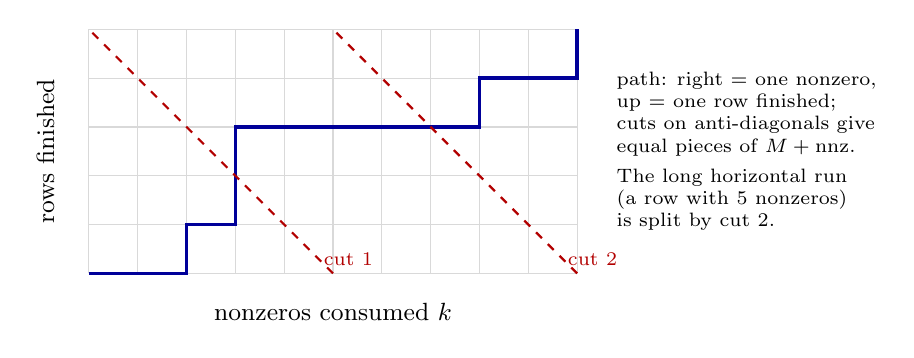
\begin{tikzpicture}[x=0.62cm, y=0.62cm, thick]

  \draw[step=1, gray!30, thin] (0,0) grid (10,5);
  \node[font=\small, anchor=north] at (5,-0.4) {nonzeros consumed $k$};
  \node[font=\small, rotate=90, anchor=south] at (-0.5,2.5) {rows finished};

  \draw[blue!60!black, very thick] (0,0) -- (2,0) -- (2,1) -- (3,1) -- (3,2) -- (3,3)
        -- (8,3) -- (8,4) -- (10,4) -- (10,5);

  \foreach \d/\c in {5/red!70!black, 10/red!70!black} {
    \draw[\c, dashed] (\d,0) -- (\d-5,5);
  }
  \node[font=\scriptsize, red!70!black, anchor=west] at (4.6,0.3) {cut 1};
  \node[font=\scriptsize, red!70!black, anchor=west] at (9.6,0.3) {cut 2};
  \node[font=\scriptsize, align=left, anchor=west] at (10.6,2.5)
    {path: right = one nonzero,\\ up = one row finished;\\ cuts on anti-diagonals give\\ equal pieces of $M+\text{nnz}$.\\[3pt] The long horizontal run\\ (a row with 5 nonzeros)\\ is split by cut 2.};
\end{tikzpicture}
\end{center}

Each thread finds the start and end of its piece by a binary search along an
anti-diagonal ($O(\log M)$). A piece can begin or end inside a row. The thread then:
\begin{itemize}
  \item stores $y_i$ for every row that \emph{ends} inside its piece (for the first row this
        may be only the tail of the row);
  \item keeps the partial sum of the row that is still open at the end of its piece as a
        \emph{carry} (\texttt{carry\_row[t]}, \texttt{carry\_val[t]}).
\end{itemize}
After the implicit barrier of the parallel region, one thread adds the $T$ carries to $y$.
A row longer than several pieces is simply split among several threads, each contributing a
carry. No locks or atomics are needed: during the parallel phase every $y_i$ is written by
one thread only, and the carries are written to separate array slots.

\subsection{Code}
\lstinputlisting[title=\texttt{spmv\_kernels.c}]{spmv_kernels.c}

\subsection{Memory placement}
\texttt{csr\_read} and \texttt{spmv\_bench} initialize every large array in parallel with
\texttt{schedule(static)} before filling it (\emph{first touch}). On a multi-socket server
this places each part of the matrix in the memory attached to the core that will use it;
on a laptop with one memory controller it has no effect but costs nothing. Threads should be
pinned with \texttt{OMP\_PROC\_BIND=close} and \texttt{OMP\_PLACES=cores}~\cite{vdp}.

\section{Correctness}
Every run of \texttt{spmv\_bench} computes $y$ with a serial reference first and compares
each kernel against it (\texttt{max error} column, relative to $\max_i|y_i|$). The tests
performed:
\begin{enumerate}
  \item The $6\times6$ running example of the notes (Sec.~2.3), stored in
        \texttt{example.mtx}, with $x=(1,\dots,6)$: all kernels give
        $y=(20,6,0,27,4,56)$, including the empty row.
  \item The converter, on a symmetric synthetic graph with 3000 vertices, against SciPy's
        Matrix Market reader: products agree to a relative error of $2\cdot10^{-15}$.
  \item All four kernels on four matrices (with empty rows, and with rows holding up to 12\%
        of all nonzeros) at 1, 2, 3, 5, 7, 16 and 33 threads: 112 runs, all with error at
        most $10^{-12}$, most exactly 0. The odd and large thread counts force the
        merge-path kernel to split rows between several threads.
\end{enumerate}
Results may differ from the serial reference in the last bits because the merge kernel adds
the pieces of a split row in a different order (notes, Sec.~9).

\section{First measurements}
The development machine (2 cores of an Intel Xeon, 7\,GB of memory) cannot hold the MAWI
matrix, so the measurements use a synthetic graph of similar type (about two nonzeros per
row, a few very long rows), made by \texttt{gen\_graph}: $M = 2\cdot10^7$, nnz $=4.2\cdot10^7$ (2.1 per row), 32\% empty rows,
and 4 hub rows that together hold 45\% of the nonzeros (the largest one 11\%).

\paragraph{Partition quality.} \texttt{spmv\_bench} prints the work of the busiest thread
divided by the average, with work $=$ rows $+$ nonzeros. It depends only on the matrix and
$T$, not on the machine:
\begin{center}
\small
\begin{tabular}{@{}lcccc@{}}
\toprule
 & $T=2$ & $T=4$ & $T=8$ & $T=16$ \\ \midrule
synthetic, hubs 3\% each: static & 1.08 & 1.25 & 1.59 & 2.27 \\
synthetic, hubs 3\% each: nnz    & 1.05 & 1.05 & 1.05 & 1.05 \\
synthetic, hubs 11\% each: static & 1.30 & -- & 3.13 & -- \\
synthetic, hubs 11\% each: nnz    & 1.26 & -- & 1.26 & -- \\
merge (any matrix)                     & 1.00 & 1.00 & 1.00 & 1.00 \\
\bottomrule
\end{tabular}
\end{center}
With 8 threads the static split gives one thread more than three times the average work, so
it cannot run faster than about $8/3.13\approx2.6$ times the serial speed.

\paragraph{Times.} Hub graph (11\% per hub), best of 10 runs:
\begin{center}
\small
\begin{tabular}{@{}lrrrr@{}}
\toprule
kernel & 1 thread (s) & 2 threads (s) & speed-up & GB/s (2 thr.) \\ \midrule
serial  & 0.490 & --    & --   & --   \\
static  & --    & 0.310 & 1.58 & 3.17 \\
dynamic & --    & 0.248 & 1.98 & 3.97 \\
nnz     & --    & 0.274 & 1.79 & 3.60 \\
merge   & --    & 0.283 & 1.73 & 3.48 \\
\bottomrule
\end{tabular}
\end{center}
Two observations:
\begin{itemize}
  \item With only 2 threads the partitions do not differ much; the static penalty grows
        with $T$ (table above). The real comparison is on a machine with more cores.
  \item The achieved bandwidth (3--4\,GB/s) is far below the machine's memory bandwidth.
        The \texttt{GB/s} column uses the \emph{best-case} traffic of the notes (Sec.~4.2),
        which assumes $x$ stays in cache. Here $x$ has $2\cdot10^7$ entries (160\,MB) and is
        read at random positions, so almost every access to $x$ misses the cache and loads a
        whole 64-byte line for 8 useful bytes: the \emph{worst case} of the notes, made
        worse by the cache line. On this kind of graph the gather from $x$, not the
        matrix, dominates the cost.
\end{itemize}

Equal \emph{work} is also not exactly equal \emph{time}: a nonzero whose $x_j$ is in cache
costs much less than one that misses. The hub rows read $x$ at random positions, while the
short rows mostly read $x_{\text{hub}}$, which stays in cache. This is why the dynamic
schedule, which reacts to the real time spent, can beat the merge split on a given machine.

\section{Running on mawi\_201512020130}
\begin{lstlisting}[style=sh]
make && make test
wget https://suitesparse-collection-website.herokuapp.com/MM/MAWI/mawi_201512020130.tar.gz
tar xzf mawi_201512020130.tar.gz
./mtx2csr mawi_201512020130/mawi_201512020130.mtx mawi_130.csr
export OMP_PROC_BIND=close OMP_PLACES=cores
for t in 1 2 4 $(nproc); do OMP_NUM_THREADS=$t ./spmv_bench mawi_130.csr 10; done
\end{lstlisting}

\paragraph{What to expect.} One product moves at least
$12\cdot2.70\cdot10^8 + 8\cdot1.29\cdot10^8\cdot3 \approx 6.3$\,GB. At a laptop memory
bandwidth of 20--40\,GB/s the roofline model (notes, Sec.~5) gives a lower bound of
0.16--0.32\,s per product; the random gather from $x$ (1\,GB, far larger than the cache)
will add to that. The things to look at in the output are:
\begin{enumerate}
  \item the \texttt{rows} line: the length of the longest row and its share of nnz;
  \item the \texttt{imbalance} line for your number of cores;
  \item how close each kernel gets to the bandwidth bound, and which split wins.
\end{enumerate}

\section{Possible improvements}
\begin{itemize}
  \item \textbf{Locality of $x$.} Reordering rows and columns (e.g.\ reverse Cuthill--McKee,
        or ordering vertices by degree) so that nearby rows read nearby entries of $x$
        attacks the dominant cost found above (notes, Sec.~7).
  \item \textbf{Pattern matrices.} For graphs without weights (kmer, GAP-kron), drop
        \texttt{val} and add $x_j$ directly: 4 instead of 12 bytes per nonzero.
  \item \textbf{SIMD.} \texttt{\#pragma omp simd reduction(+:s)} on the inner loop; limited
        by the gather and the short rows (notes, Sec.~8.3; van der Pas et al.~\cite{vdp}).
  \item \textbf{Validation against a library}, such as Intel MKL's
        \texttt{mkl\_sparse\_d\_mv}, for both correctness and speed (notes, Sec.~10).
\end{itemize}

\begin{keyidea}
\begin{itemize}
  \item At $10^8$ rows, index width, memory budget and file conversion are design decisions
        in their own right.
  \item The kernels differ only in the work split. The merge path balances rows and
        nonzeros exactly and splits long rows, with a carry fix-up instead of locks.
  \item For irregular graphs the random gather from $x$ dominates: the measured bandwidth is
        far below the best-case model, so data locality matters more than the arithmetic.
\end{itemize}
\end{keyidea}

\begin{thebibliography}{9}
\bibitem{notes} G.~Lozano. \emph{Matrix--Vector Multiplication $y=Ax$: Dense versus CSR
  Storage}. Notes, November 2026.
\bibitem{merrill} D.~Merrill and M.~Garland. Merge-based parallel sparse matrix--vector
  multiplication. In \emph{Proceedings of SC16}, 2016.
\bibitem{suitesparse} T.~A.~Davis and Y.~Hu. The University of Florida sparse matrix
  collection. \emph{ACM Transactions on Mathematical Software}, 38(1):1--25, 2011.
  \url{https://sparse.tamu.edu}
\bibitem{mm} R.~F. Boisvert, R.~Pozo, and K.~A. Remington. The Matrix Market exchange
  formats: initial design. NISTIR 5935, NIST, 1996.
\bibitem{chapman} B.~Chapman, G.~Jost, and R.~van der Pas. \emph{Using OpenMP: Portable
  Shared Memory Parallel Programming}. MIT Press, Cambridge, MA, 2007.
\bibitem{vdp} R.~van der Pas, E.~Stotzer, and C.~Terboven. \emph{Using OpenMP --- The Next
  Step: Affinity, Accelerators, Tasking, and SIMD}. MIT Press, Cambridge, MA, 2017.
\end{thebibliography}
\end{document}
